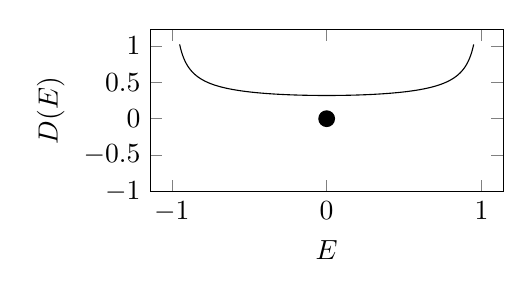
\begin{tikzpicture}
    \begin{axis}[
            xlabel={$E$},
            ylabel={$D(E)$},
            width=0.5\linewidth,
            height=0.3\linewidth,
            samples=300,
            domain=-0.95:0.95,
            ymin=-1,
        ]

        \addplot[black] {abs(sqrt(0.5 + 0.5*(2*x^2-1))/(3.141*x*sqrt(1 - x^2)))};
        \node[circle, draw=black, fill=black, inner sep=2pt] at (axis cs:0, 0) {};
    \end{axis}

\end{tikzpicture}
